\documentclass[11pt, aspectratio=169]{beamer}
% \documentclass[11pt,handout]{beamer}
\usepackage[T1]{fontenc}
\usepackage[utf8]{inputenc}
\usepackage{textcomp}
\usepackage{float, afterpage, rotating, graphicx}
\usepackage{epstopdf}
\usepackage{longtable, booktabs, tabularx}
\usepackage{fancyvrb, moreverb, relsize}
\usepackage{eurosym, calc}
\usepackage{amsmath, amssymb, amsfonts, amsthm, bm}
\usepackage[
    natbib=true,
    bibencoding=inputenc,
    bibstyle=authoryear-ibid,
    citestyle=authoryear-comp,
    maxcitenames=3,
    maxbibnames=10,
    useprefix=false,
    sortcites=true,
    backend=biber
]{biblatex}
\AtBeginDocument{\toggletrue{blx@useprefix}}
\AtBeginBibliography{\togglefalse{blx@useprefix}}
\setlength{\bibitemsep}{1.5ex}
\addbibresource{refs.bib}

\hypersetup{colorlinks=true, linkcolor=black, anchorcolor=black, citecolor=black, filecolor=black, menucolor=black, runcolor=black, urlcolor=black}

\setbeamertemplate{footline}[frame number]
\setbeamertemplate{navigation symbols}{}
\setbeamertemplate{frametitle}{\centering\vspace{1ex}\insertframetitle\par}


\begin{document}

\title{shrinkage_python}

\author[Klaus Aulbach]
{
{\bf Klaus Aulbach}\\
{\small University of Bonn }\\[1ex]
}


\begin{frame}
    \titlepage
    \note{~}
\end{frame}


\begin{frame}[t]
    \frametitle{heading here}
    \begin{itemize}
        \item<+-> Please cite this template as: \citet{GaudeckerEconProjectTemplates}
        \item<+-> Example data is taken from \url{https://www.stem.org.uk/resources/elibrary/resource/28452/large-datasets-stats4schools}
    \end{itemize}
    \note{~}
\end{frame}



\begin{frame}[t]
    \begin{figure}[H]

        \centering
        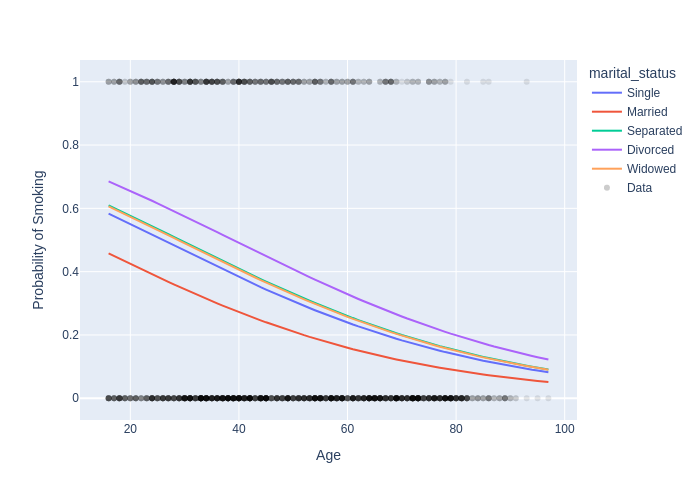
\includegraphics[width=0.5\textwidth]{../figures/smoking_by_marital_status}

        \caption{\emph{Python:} Model predictions of the smoking probability over the
            lifetime. Each colored line represents a case where marital status is fixed to
            one of the values present in the data set.}
        \label{fig:python-predictions}

    \end{figure}
\end{frame}



% Print black screen only in presentation mode for finishing up.
\mode<beamer> {
    \beamersetaveragebackground{black}
    \begin{frame}
        \frametitle{}
    \end{frame}

    \beamersetaveragebackground{white}
}

\begin{frame}[allowframebreaks]
    \frametitle{References}
    \renewcommand{\bibfont}{\normalfont\footnotesize}
    \printbibliography
\end{frame}

\end{document}
